\documentclass[a4paper,11pt]{article}
\usepackage{graphicx}
\usepackage[utf8]{inputenc}
\usepackage{hyperref}
\usepackage{placeins}
\usepackage[newfloat]{minted}
\usepackage{caption}

\newenvironment{code}{\captionsetup{type=listing}}{}
\SetupFloatingEnvironment{listing}{name=Code Overview}


\hypersetup{
    colorlinks=true,
    linkcolor=blue,
    filecolor=black,      
    urlcolor=blue,
    citecolor=black,
}
\begin{document}

\title{
    \textbf{Trees Report.}
}
\author{Adrian Jonsson Sjödin}
\date{Fall 2022}

\maketitle

\section{Introduction}
In this assignment we will take a closer look at \textit{tree} structures, and in
particular at tree structure called \textit{binary search trees}. The operations that we will look at and
implement are: construction, adding and searching for and removing an item.

\section{Task}
Implement a binary search tree structure that is ordered with smaller keys to the left and create the
following two methods:
\begin{itemize}
    \item {\tt add(Integer key, Integer value)}: adds a new node (leaf) to the
          tree that maps the key to the value. If the key is already present we
          update the value of the node.
    \item {\tt lookup(Integer key)}: find and return the value associate to the
          key. If the key is not found we return null.
\end{itemize}
benchmark the lookup algorithm and compare it to the benchmark of the binary search algorithm that
was done in a previous assignment.

Also create an iterator that we can use to traverse the tree. The iterator should implements Java's
Iterator class and override the {\tt hasNext()} and {\tt next()} method. Explain how you implemented
the methods of the tree iterator class. Also describe what will happen if you create an iterator,
retrieve a few elements and then add new elements to the tree. Will it work, what is the state of the
iterator, will we lose values?

\section{Method \& Theory}
This data structure is called a \textit{tree} since the structure originates in a root from where we
spread out into branches, that then in turn can further divide into their own branches. A branch that
does not divide further is terminated by a so called leaf.

A \textit{binary search tree} is a tree whose branch always divides into two branches, unless it terminates
into a leaf.
\subsection{Lookup}

I won't show the code for how the {\tt BinaryTree} class is constructed here since it
is already explained in the assignment, I will instead focus on the {\tt add()} and
    {\tt lookup()} method. When we create a binary search tree we initialize it empty, i.e. the
root is set to null. The first node we add to the tree will then become the root, and
all subsequent nodes will then be added recursively down left or right of the root
depending on the node's key. If the key-value pair we want to add already exists in the
tree we instead change the value of that key-value pair to the new value. This ensures
that all key-value pairs are unique. Code overview \ref{code:add} shows how this work.

The {\tt lookup()} method however is not recursive, instead it uses a while loop to look
at each node, see if it is the key we want and if not go down left or right in the tree
depending on the current node's key size. It does this until we find the key we are looking
for, or we reach a null pointer in which case the key we're looking for doesn't exist in
the tree. The {\tt lookup} method can be seen in code overview \ref{code:lookup}.

This way of searching should give us a time complexity of $\mathcal{O}(h)$ where
$h$ is the height of tree. For a balanced tree (the height difference of nodes on
left and right subtree is not more than one) the height becomes $log(n)$, where $n$ is
the number of nodes in the tree. That means we should see a time complexity of
$\mathcal{O}(log(n))$ in our benchmark of the {\tt lookup()} method.

\subsection{Iterator}
To implement the iterator I first had to modify my {\tt Stack} class so that it could
handle nodes as well. This because the dynamic stack we implemented in a previous assignment
was only able to handle the {\tt int} primitive data structure. Instead of simply modifying
it to be able to handle nodes I went with creating a dynamic array stack that could handle
any generic object so that we can potentially reuse it in coming assignment.

The iterator itself was implement according to the instructions provided. That is I implemented
the two methods {\tt next()} and {\tt hasNext}, and made {\tt next()} move through the tree
from the bottommost left node and upwards in increasing key size order. To do this we
created a private method called {\tt moveLeft(Node current)} that will move down left
through the tree and push each node to the stack. When we then call the {\tt Iterator}
we return a new {\tt TreeIterator} whose constructor takes in the current {\tt root} of
the tree as a parameter and creates a stack. It also calls the private {\tt moveLeft}
method which will traverse the tree from the root down to the bottommost left node and
push each node to the stack. When we then call the {\tt next} method for the first time
we will then start at the bottom with the node containing the smallest key at the top of
the stack, and with the pointer called current pointing the that node's left which would
be null.

The {\tt next} method itself works as following: We start with checking if there is a next node
in the tree whose value we can retrieve. This is done with the {\tt hasNext} method that
checks whether or not the stack is empty. If it is empty that means we have traversed the
whole tree and an exception is thrown. Otherwise we pop the stack and set current to
be the popped node. We then check if that node has any branches down right. If it has we
call the {\tt moveLeft} method which will push that right branch's left branches to the
stack. This way the next node popped when we call {\tt next()} again will always be the
node whose key is the smallest. After that is done we return the value that is stored in the
popped node.

The code for {\tt next()} and {\tt moveLeft(Node current)} can be seen in code overview
\ref{code:iterator}.


\section{Result}
The result from the benchmark of the {\tt lookup()} method can be seen in figure \ref{fig:bench}.
In it we measure how long one long it takes to search for one random key from a tree
populated by $\sim4,000,000$ million random keys, and double the size of the tree for every measurement.
\begin{figure}[h!]
    \centering
    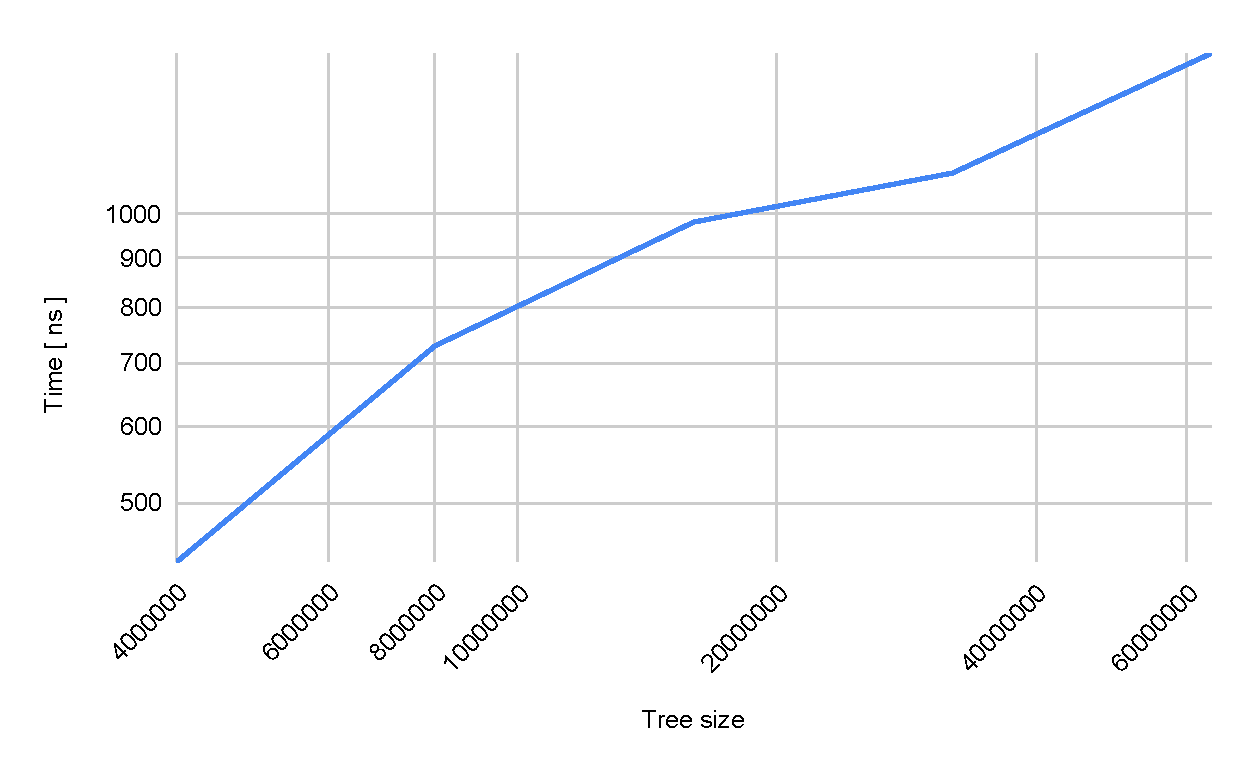
\includegraphics[width=.8\textwidth]{benchmarkData.pdf}
    \caption{Benchmark data for the {\tt lookup()} method}
    \label{fig:bench}
\end{figure}
\newpage
\section{Discussion}
As seen in figure \ref{fig:bench} the graph is somewhat linear in a log-log scale, which
indicates that our statement above about it being of time complexity $\mathcal{O}(log(n))$
is promising. The reason why the graph is somewhat skewed and not quite linear is
probably because in each benchmark a new tree with random branches are created and
we're searching for a random key. That means it is possible for some measurements to be
faster if we're lucky and the key we are searching for is closer to the root, than it
is in a smaller tree which then will take longer to search. With this in mind I feel
that the data is confirming my statement about the time complexity.

This also means that looking up a key in a binary search tree is on the same order of magnitude
that it takes to search for an element in a sorted array with binary search. This however 
doesn't come as a surprise since a binary search tree is created off of the same principle as 
the binary search algorithm, allowing us to skip about half the tree on average for each comparison.

The iterator works as intended and if you start retrieving a few values with it before adding more nodes
to the tree the {\tt next} method will retrieve them as well, as long as the iterator hasn't already passed 
the position where that node will be created. If it has then the {\tt next} method will of course not retrieve
them since they are behind where the pointer in {\tt next} is pointing. However they will be retrieved if we use
an enhanced for each loop after it since it creates a new separate local instance of an iterator that will start at the 
bottom of the tree and traverse it depth first.

So in conclusion adding new nodes to the tree after already staring to retrieve elements will not affect the iterator 
negatively and neither will we lose values. 

\newpage
\FloatBarrier
\section*{Code}
All the code can be found here: \href{https://github.com/adrian-jonsson-sjoedin/ID1021-AlgoData/tree/main/Tasks/Trees/src}{GitHub}

\begin{code}
    \captionof{listing}{Add to binary search tree}
    \label{code:add}
    \begin{minted}{java}
public void add(Integer k, Integer v) {
    if (root == null) {
        root = new Node(k, v);
    } else {
        root.add(k, v);
    }
}        
private void add(Integer k, Integer v) {
if (this.key == k) {
    this.value = v;
}
if (this.key > k) {
    if (this.left == null) {
        this.left = new Node(k, v);
    } else {
        this.left.add(k, v);
    }
} else {
    if (this.right == null) {
        this.right = new Node(k, v);
    } else {
        this.right.add(k, v);
    }
}
}
\end{minted}
\end{code}
\begin{code}
    \captionof{listing}{Look up key in binary search tree}
    \label{code:lookup}
    \begin{minted}{java}
public Integer lookup(Integer key) {
    return root.lookup(key);
}
private Integer lookup(Integer k) {
    Node current = this;
    while (current != null) {
        if (current.key == k) {
            return current.value;
        } else if (current.key > k) {
            current = current.left;
        } else {
            current = current.right;
        }
    }
    return null;
}
\end{minted}
\end{code}

\begin{code}
    \captionof{listing}{{\tt Next()} and {\tt moveLeft(Node current)}}
    \label{code:iterator}
    \begin{minted}{java}
private void moveLeft(Node current) {
    while (current != null) {
        stack.push(current);
        current = current.left;
    }
}
@Override
public Integer next() {
    if (!hasNext()) {
        throw new NoSuchElementException();
    }
    Node curr = stack.pop();
    if (curr.right != null) {
        moveLeft(curr.right);
    }
    next = curr;
    return curr.value;
}
\end{minted}
\end{code}
\end{document}
